\chapter{行列}
\section{行列とは}
\emph{行列}\index{ぎょうれつ@行列}は、単純には数字を縦横に並べただけのものである。ただ、行列に対して様々な演算を組み込むことで、数学や物理学上非常に有用な概念となる。
\begin{definition*}{行列}
	\emph{行列}は数字を縦横にいくつか並べたものである。以下のように、縦に\(m\)個、横に\(n\)個数字を並べた行列
	\begin{equation}
		\boldsymbol{A}=
		\begin{pmatrix}
			a_{11} & a_{12} & \dots  & a_{1n} \\
			a_{21} & a_{22} & \dots  & a_{2n} \\
			\vdots & \vdots & \ddots & \vdots \\
			a_{m1} & a_{m2} & \dots  & a_{mn} \\
		\end{pmatrix}
	\end{equation}
	を\(m\times n\)行列と呼び、特に\(m=n\)の行列を(\(n\)次の)\emph{正方行列}\index{せいほうぎょうれつ@正方行列}と呼ぶ。並べられた数字を\emph{成分}と呼び、\(a_{ij}\)を\((i,j)\)成分などと呼ぶ。
\end{definition*}
一般的に、1つ目の添字が行番号を、2つ目の添字が列番号を示す場合が多い。
\section{3次正方行列}
物理的には\(3\times 3\)の正方行列(3次正方行列)が非常に重要である。これは後述する2階のテンソルを表現することができるためである。\(3\times 3\)の正方行列は以下のように9つの成分を縦横に並べたものである。
\begin{definition*}{3次正方行列}
	3次正方行列は数字を9つ並べたものである。
	\begin{equation}
		\boldsymbol{A}=
		\begin{pmatrix}
			a_{11} & a_{12} & a_{13} \\
			a_{21} & a_{22} & a_{23} \\
			a_{31} & a_{32} & a_{33} \\
		\end{pmatrix}
	\end{equation}
\end{definition*}

\subsection{行列の和とスカラー倍}
3次正方行列のスカラー倍および和は単純に、各成分のスカラー倍と和によって計算される。
\begin{definition*}{3次正方行列のスカラー倍}
	3次正方行列\(\boldsymbol{A}\)の定数\(k\)倍は各成分を\(k\)倍し、
	\begin{equation}
		k\boldsymbol{A}=
		\begin{pmatrix}
			ka_{11} & ka_{12} & ka_{13} \\
			ka_{21} & ka_{22} & ka_{23} \\
			ka_{31} & ka_{32} & ka_{33} \\
		\end{pmatrix}
	\end{equation}
	と定義される。
\end{definition*}
\begin{definition*}{3次正方行列の和}
	3次正方行列\(\boldsymbol{A},\boldsymbol{B}\)の和は各成分を足し合わせ
	\begin{equation}
		\boldsymbol{A}+\boldsymbol{B}=
		\begin{pmatrix}
			a_{11}+b_{11} & a_{12}+b_{12}   & a_{13}+b_{13}  \\
			a_{21}+b_{21} & a_{22} + b_{22} & a_{23} +b_{23} \\
			a_{31}+b_{31} & a_{32} + b_{32} & a_{33} +b_{33} \\
		\end{pmatrix}
	\end{equation}
	とする。
\end{definition*}
\subsection{行列積}
行列積\index{ぎょうれつせき@行列積}は、いくつかの種類が考えられる。ただし、普通行列積と言う際には以下の積を示す。
\begin{definition*}{3次正方行列の積}
	3次正方行列\(\boldsymbol{A},\boldsymbol{B}\)の積\(\boldsymbol{AB}\)は
	\begin{equation}
		\boldsymbol{A}\boldsymbol{B}=
		\begin{pmatrix}
			a_{11}b_{11}+a_{12}b_{21} +a_{13}b_{31} & a_{11}b_{12}+a_{12}b_{22} +a_{13}b_{32} & a_{11}b_{13}+a_{12}b_{23} +a_{13}b_{33} \\
			a_{21}b_{11}+a_{22}b_{21} +a_{23}b_{31} & a_{21}b_{12}+a_{22}b_{22} +a_{23}b_{32} & a_{21}b_{13}+a_{22}b_{23} +a_{23}b_{33} \\
			a_{31}b_{11}+a_{32}b_{21} +a_{33}b_{31} & a_{31}b_{12}+a_{32}b_{22} +a_{33}b_{32} & a_{31}b_{13}+a_{32}b_{23} +a_{33}b_{33} \\
		\end{pmatrix}
	\end{equation}
	のように計算する。これは、\(\boldsymbol{AB}\)の\((i,j)\)成分を\((\boldsymbol{A}\boldsymbol{B})_{ij}\)と書くとすれば、
	\begin{equation}
		(\boldsymbol{A}\boldsymbol{B})_{ij}=a_{i1}b_{1j}+a_{i2}b_{2j}+a_{i3}b_{3j}=\sum_{k=1}^{3} a_{ik}b_{kj}
	\end{equation}
	とも書ける。
\end{definition*}
このような一見複雑な形の積が行列積として広く用いられている理由は、この形がベクトルの一次変換の合成として現れるためである。すなわち、ベクトル\(\boldsymbol{v}\)を\(\boldsymbol{v}'\)に一次変換する行列\(\boldsymbol{A}\)を考えると、これは
\begin{equation}
	\boldsymbol{v}'=\boldsymbol{A}\boldsymbol{v}
\end{equation}
を満たす。これに対して\(\boldsymbol{v}'\)を更に変換し\(\boldsymbol{v}''\)に変換する行列\(\boldsymbol{B}\)は
\begin{equation}
	\boldsymbol{v}''=\boldsymbol{B}\boldsymbol{v}'
\end{equation}
となる。すると、\(\boldsymbol{v}\)と\(\boldsymbol{v}''\)の関係は
\begin{equation}
	\boldsymbol{v}''=\boldsymbol{B}(\boldsymbol{A}\boldsymbol{v})
\end{equation}
となるはずである。この時、もしこれを
\begin{equation}
	\boldsymbol{v}''=(\boldsymbol{B}\boldsymbol{A})\boldsymbol{v}
\end{equation}
とできれるのであれば、\(\boldsymbol{B}\boldsymbol{A}\)を計算すれば\(\boldsymbol{v}'\)を経ることなく\(\boldsymbol{v}\)を\(\boldsymbol{v}''\)に変換できる。このように、\(\boldsymbol{B}\)による変換と\(\boldsymbol{A}\)による変換を組合わせた変換が\(\boldsymbol{B}\boldsymbol{A}\)による変換と等しくなるような\(\boldsymbol{B}\boldsymbol{A}\)の計算手法が、この行列積である。
\subsubsection{行列積の結合則}
行列積は、結合則が成立する。
\begin{theorem*}{3次正方行列積の結合則}
	3次正方行列\(\boldsymbol{A},\boldsymbol{B},\boldsymbol{C}\)の積は、どちらを先に計算しても同じであるため、括弧を付けなくてもよい。
	\begin{equation}
		(\boldsymbol{A}\boldsymbol{B})\boldsymbol{C}=\boldsymbol{A}(\boldsymbol{B}\boldsymbol{C})=\boldsymbol{A}\boldsymbol{B}\boldsymbol{C}
	\end{equation}
\end{theorem*}
\begin{proof}
	\((i,j)\)成分について\(((\boldsymbol{A}\boldsymbol{B})\boldsymbol{C})_{ij}\)と\((\boldsymbol{A}(\boldsymbol{B}\boldsymbol{C}))_{ij}\)が一致することを示せばよい。まず、\((\boldsymbol{A}\boldsymbol{B})\boldsymbol{C}\)について、
	\begin{equation}
		(\boldsymbol{A}\boldsymbol{B})_{ij}=\sum_{k=1}^{3} a_{ik}b_{kj}
	\end{equation}
	より、
	\begin{equation}
		((\boldsymbol{A}\boldsymbol{B})\boldsymbol{C})_{ij}
		=\sum_{s=1}^{3} \left((\boldsymbol{A}\boldsymbol{B})_{is}c_{sj}\right)
		=\sum_{s=1}^{3} \left(\sum_{k=1}^{3} \left(a_{ik}b_{ks} \right)c_{sj}\right)
		=\sum_{s=1}^{3} \sum_{k=1}^{3} \left(a_{ik}b_{ks}c_{sj}\right)
	\end{equation}
	である。これに対し、\(\boldsymbol{A}(\boldsymbol{B}\boldsymbol{C})\)については
	\begin{equation}
		(\boldsymbol{B}\boldsymbol{C})_{ij}=\sum_{k=1}^{3} b_{ik}c_{kj}
	\end{equation}
	より
	\begin{equation}
		(\boldsymbol{A}(\boldsymbol{B}\boldsymbol{C}))_{ij}
		=\sum_{s=1}^{3} \left(a_{is}(\boldsymbol{B}\boldsymbol{C})_{sj}\right)
		=\sum_{s=1}^{3} \left(a_{is}\sum_{k=1}^{3} \left(b_{sk}c_{kj}\right)\right)
		=\sum_{s=1}^{3} \sum_{k=1}^{3} \left(a_{is} b_{sk}c_{kj}\right)
	\end{equation}
	ここで足し合わせの添字\(k,s\)を置き換えれば(\(k=s,s=k)\)、
	\begin{equation}
		(\boldsymbol{A}(\boldsymbol{B}\boldsymbol{C}))_{ij}
		=\sum_{k=1}^{3} \sum_{s=1}^{3} \left(a_{ik} b_{ks}c_{sj}\right)
	\end{equation}
	これは\(((\boldsymbol{A}\boldsymbol{B})\boldsymbol{C})_{ij}\)と足し合わせの順番が異なるだけの全く同じ値である。よって、\(((\boldsymbol{A}\boldsymbol{B})\boldsymbol{C})_{ij}=(\boldsymbol{A}(\boldsymbol{B}\boldsymbol{C}))_{ij}\)が示された。これがすべての\((i,j)\)成分に成立するため、
	\begin{equation}
		(\boldsymbol{A}\boldsymbol{B})\boldsymbol{C}=\boldsymbol{A}(\boldsymbol{B}\boldsymbol{C})
	\end{equation}
	が示される。
\end{proof}
\subsubsection{行列積の分配則}
行列積には分配法則も成立する。
\begin{theorem*}{3次正方行列積の分配則}
	3次正方行列\(\boldsymbol{A},\boldsymbol{B},\boldsymbol{C}\)について、以下の等式が成立する。
	\begin{equation}
		\boldsymbol{A}(\boldsymbol{B}+\boldsymbol{C})=\boldsymbol{A}\boldsymbol{B}+\boldsymbol{A}\boldsymbol{C}
	\end{equation}
\end{theorem*}
\begin{proof}
	左辺の\((i,j)\)成分について
	\begin{equation}
		(\boldsymbol{A}(\boldsymbol{B}+\boldsymbol{C}))_{ij}
		=\sum_{k=1}^{3}\left( a_{ik}(b_{kj}+c_{kj})\right)
		=\sum_{k=1}^{3}\left( a_{ik}b_{kj}\right)+\sum_{k=1}^{3}\left( a_{ik}c_{kj}\right)
		=(\boldsymbol{A}\boldsymbol{B})_{ij}+(\boldsymbol{A}\boldsymbol{C})_{ij}
	\end{equation}
	より、成立する。
\end{proof}
\subsubsection{行列積の交換}
行列積では注意すべきことに可換則(交換法則)が成立しない。
\begin{theorem*}{3次正方行列積の交換}
	3次正方行列\(\boldsymbol{A},\boldsymbol{B}\)について、\(\boldsymbol{A}\boldsymbol{B}\)と\(\boldsymbol{B}\boldsymbol{A}\)は等しいとは限らない。すなわち
	\begin{equation}
		\boldsymbol{A}\boldsymbol{B}\not\equiv\boldsymbol{B}\boldsymbol{A}
	\end{equation}
	である。
\end{theorem*}
ここで、\(\not \equiv\)は「等しいとは限らない」という意味で用いた。この特徴は、\(\boldsymbol{A}\)による変換の後\(\boldsymbol{B}\)による変換をするのと、\(\boldsymbol{B}\)による変換の後\(\boldsymbol{A}\)による変換をするのでは結果が異なるというふうに捉えることもできる。たとえば、\(\boldsymbol{A}\)を「ベクトルをx軸を中心に90度回転させる変換」、\(\boldsymbol{B}\)を「ベクトルをy軸に対して90度回転させる変換」と考え、\(y\)方向の単位ベクトルを変換させることを考えれば、変換の順番によって結果が変わることがわかる\footnote{ここではこれらの変換が一次変換(線形変換)であることを示さずに例を挙げたが、これらの変換は
	\begin{equation}
		\boldsymbol{A}=\begin{pmatrix}
			1 & 0 & 0  \\
			0 & 0 & -1 \\
			0 & 1 & 0
		\end{pmatrix},
		\boldsymbol{B}=\begin{pmatrix}
			0  & 0 & 1 \\
			0  & 1 & 0 \\
			-1 & 0 & 0
		\end{pmatrix}
	\end{equation}
	で表すことができる一次変換である。
}。

\begin{figure}[ht]
	\centering
	\tikzset{every picture/.style={line width=0.75pt}} %set default line width to 0.75pt
	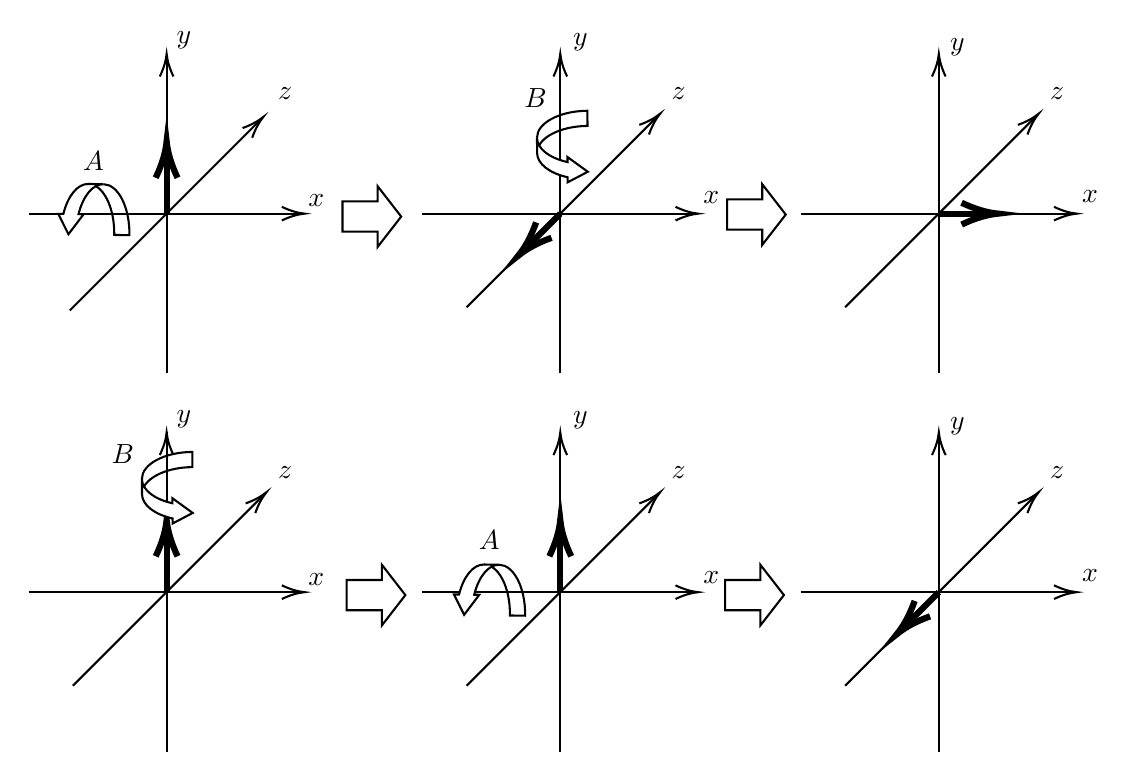
\begin{tikzpicture}[x=0.75pt,y=0.75pt,yscale=-1,xscale=1]
		%uncomment if require: \path (0,369); %set diagram left start at 0, and has height of 369
		%Straight Lines [id:da3956637324263075]
		\draw    (23.81,140.26) -- (115.67,48.41) ;
		\draw [shift={(117.08,46.99)}, rotate = 495] [color={rgb, 255:red, 0; green, 0; blue, 0 }  ][line width=0.75]    (10.93,-3.29) .. controls (6.95,-1.4) and (3.31,-0.3) .. (0,0) .. controls (3.31,0.3) and (6.95,1.4) .. (10.93,3.29)   ;
		%Straight Lines [id:da7965819303139063]
		\draw    (70.45,170.63) -- (70.45,18.63) ;
		\draw [shift={(70.45,16.63)}, rotate = 450] [color={rgb, 255:red, 0; green, 0; blue, 0 }  ][line width=0.75]    (10.93,-3.29) .. controls (6.95,-1.4) and (3.31,-0.3) .. (0,0) .. controls (3.31,0.3) and (6.95,1.4) .. (10.93,3.29)   ;
		%Straight Lines [id:da8389984930075898]
		\draw    (4,93.63) -- (134.89,93.63) ;
		\draw [shift={(136.89,93.63)}, rotate = 180] [color={rgb, 255:red, 0; green, 0; blue, 0 }  ][line width=0.75]    (10.93,-3.29) .. controls (6.95,-1.4) and (3.31,-0.3) .. (0,0) .. controls (3.31,0.3) and (6.95,1.4) .. (10.93,3.29)   ;
		%Straight Lines [id:da18173005600967795]
		\draw [line width=2.25]    (70.45,93.63) -- (70.45,62.84) ;
		\draw [shift={(70.45,58.84)}, rotate = 450] [color={rgb, 255:red, 0; green, 0; blue, 0 }  ][line width=2.25]    (17.49,-5.26) .. controls (11.12,-2.23) and (5.29,-0.48) .. (0,0) .. controls (5.29,0.48) and (11.12,2.23) .. (17.49,5.26)   ;
		%Straight Lines [id:da08112513112728958]
		\draw    (214.97,138.72) -- (306.83,46.86) ;
		\draw [shift={(308.24,45.45)}, rotate = 495] [color={rgb, 255:red, 0; green, 0; blue, 0 }  ][line width=0.75]    (10.93,-3.29) .. controls (6.95,-1.4) and (3.31,-0.3) .. (0,0) .. controls (3.31,0.3) and (6.95,1.4) .. (10.93,3.29)   ;
		%Straight Lines [id:da9675110345407418]
		\draw    (260.11,170.63) -- (260.11,18.63) ;
		\draw [shift={(260.11,16.63)}, rotate = 450] [color={rgb, 255:red, 0; green, 0; blue, 0 }  ][line width=0.75]    (10.93,-3.29) .. controls (6.95,-1.4) and (3.31,-0.3) .. (0,0) .. controls (3.31,0.3) and (6.95,1.4) .. (10.93,3.29)   ;
		%Straight Lines [id:da6600835675219325]
		\draw    (193.67,93.63) -- (324.56,93.63) ;
		\draw [shift={(326.56,93.63)}, rotate = 180] [color={rgb, 255:red, 0; green, 0; blue, 0 }  ][line width=0.75]    (10.93,-3.29) .. controls (6.95,-1.4) and (3.31,-0.3) .. (0,0) .. controls (3.31,0.3) and (6.95,1.4) .. (10.93,3.29)   ;
		%Straight Lines [id:da4809736183174831]
		\draw [line width=2.25]    (260.11,93.63) -- (242.65,111.1) ;
		\draw [shift={(239.82,113.93)}, rotate = 315] [color={rgb, 255:red, 0; green, 0; blue, 0 }  ][line width=2.25]    (17.49,-5.26) .. controls (11.12,-2.23) and (5.29,-0.48) .. (0,0) .. controls (5.29,0.48) and (11.12,2.23) .. (17.49,5.26)   ;
		%Straight Lines [id:da41361996262409906]
		\draw    (397.34,138.72) -- (489.2,46.86) ;
		\draw [shift={(490.61,45.45)}, rotate = 495] [color={rgb, 255:red, 0; green, 0; blue, 0 }  ][line width=0.75]    (10.93,-3.29) .. controls (6.95,-1.4) and (3.31,-0.3) .. (0,0) .. controls (3.31,0.3) and (6.95,1.4) .. (10.93,3.29)   ;
		%Straight Lines [id:da4151818121512938]
		\draw    (442.49,170.63) -- (442.49,18.63) ;
		\draw [shift={(442.49,16.63)}, rotate = 450] [color={rgb, 255:red, 0; green, 0; blue, 0 }  ][line width=0.75]    (10.93,-3.29) .. controls (6.95,-1.4) and (3.31,-0.3) .. (0,0) .. controls (3.31,0.3) and (6.95,1.4) .. (10.93,3.29)   ;
		%Straight Lines [id:da7267472416419822]
		\draw    (376.04,93.63) -- (506.93,93.63) ;
		\draw [shift={(508.93,93.63)}, rotate = 180] [color={rgb, 255:red, 0; green, 0; blue, 0 }  ][line width=0.75]    (10.93,-3.29) .. controls (6.95,-1.4) and (3.31,-0.3) .. (0,0) .. controls (3.31,0.3) and (6.95,1.4) .. (10.93,3.29)   ;
		%Straight Lines [id:da6810501209045401]
		\draw [line width=2.25]    (442.49,93.63) -- (466.96,93.63) ;
		\draw [shift={(470.96,93.63)}, rotate = 180] [color={rgb, 255:red, 0; green, 0; blue, 0 }  ][line width=2.25]    (17.49,-5.26) .. controls (11.12,-2.23) and (5.29,-0.48) .. (0,0) .. controls (5.29,0.48) and (11.12,2.23) .. (17.49,5.26)   ;
		%Straight Lines [id:da9408310523996324]
		\draw    (25.3,321.09) -- (117.16,229.24) ;
		\draw [shift={(118.57,227.82)}, rotate = 495] [color={rgb, 255:red, 0; green, 0; blue, 0 }  ][line width=0.75]    (10.93,-3.29) .. controls (6.95,-1.4) and (3.31,-0.3) .. (0,0) .. controls (3.31,0.3) and (6.95,1.4) .. (10.93,3.29)   ;
		%Straight Lines [id:da17249684905242657]
		\draw    (70.45,353) -- (70.45,201.01) ;
		\draw [shift={(70.45,199.01)}, rotate = 450] [color={rgb, 255:red, 0; green, 0; blue, 0 }  ][line width=0.75]    (10.93,-3.29) .. controls (6.95,-1.4) and (3.31,-0.3) .. (0,0) .. controls (3.31,0.3) and (6.95,1.4) .. (10.93,3.29)   ;
		%Straight Lines [id:da8074046458367652]
		\draw    (4,276) -- (134.89,276) ;
		\draw [shift={(136.89,276)}, rotate = 180] [color={rgb, 255:red, 0; green, 0; blue, 0 }  ][line width=0.75]    (10.93,-3.29) .. controls (6.95,-1.4) and (3.31,-0.3) .. (0,0) .. controls (3.31,0.3) and (6.95,1.4) .. (10.93,3.29)   ;
		%Straight Lines [id:da06875717034690143]
		\draw [line width=2.25]    (70.45,276) -- (70.45,245.21) ;
		\draw [shift={(70.45,241.21)}, rotate = 450] [color={rgb, 255:red, 0; green, 0; blue, 0 }  ][line width=2.25]    (17.49,-5.26) .. controls (11.12,-2.23) and (5.29,-0.48) .. (0,0) .. controls (5.29,0.48) and (11.12,2.23) .. (17.49,5.26)   ;
		%Straight Lines [id:da14028894750223952]
		\draw    (214.97,321.09) -- (306.83,229.24) ;
		\draw [shift={(308.24,227.82)}, rotate = 495] [color={rgb, 255:red, 0; green, 0; blue, 0 }  ][line width=0.75]    (10.93,-3.29) .. controls (6.95,-1.4) and (3.31,-0.3) .. (0,0) .. controls (3.31,0.3) and (6.95,1.4) .. (10.93,3.29)   ;
		%Straight Lines [id:da07623113782042457]
		\draw    (260.11,353) -- (260.11,201.01) ;
		\draw [shift={(260.11,199.01)}, rotate = 450] [color={rgb, 255:red, 0; green, 0; blue, 0 }  ][line width=0.75]    (10.93,-3.29) .. controls (6.95,-1.4) and (3.31,-0.3) .. (0,0) .. controls (3.31,0.3) and (6.95,1.4) .. (10.93,3.29)   ;
		%Straight Lines [id:da7609078821857935]
		\draw    (193.67,276) -- (324.56,276) ;
		\draw [shift={(326.56,276)}, rotate = 180] [color={rgb, 255:red, 0; green, 0; blue, 0 }  ][line width=0.75]    (10.93,-3.29) .. controls (6.95,-1.4) and (3.31,-0.3) .. (0,0) .. controls (3.31,0.3) and (6.95,1.4) .. (10.93,3.29)   ;
		%Straight Lines [id:da12851034928346516]
		\draw    (397.34,321.09) -- (489.2,229.24) ;
		\draw [shift={(490.61,227.82)}, rotate = 495] [color={rgb, 255:red, 0; green, 0; blue, 0 }  ][line width=0.75]    (10.93,-3.29) .. controls (6.95,-1.4) and (3.31,-0.3) .. (0,0) .. controls (3.31,0.3) and (6.95,1.4) .. (10.93,3.29)   ;
		%Straight Lines [id:da879156352596987]
		\draw    (442.49,353) -- (442.49,201.01) ;
		\draw [shift={(442.49,199.01)}, rotate = 450] [color={rgb, 255:red, 0; green, 0; blue, 0 }  ][line width=0.75]    (10.93,-3.29) .. controls (6.95,-1.4) and (3.31,-0.3) .. (0,0) .. controls (3.31,0.3) and (6.95,1.4) .. (10.93,3.29)   ;
		%Straight Lines [id:da2250988447742288]
		\draw    (376.04,276) -- (506.93,276) ;
		\draw [shift={(508.93,276)}, rotate = 180] [color={rgb, 255:red, 0; green, 0; blue, 0 }  ][line width=0.75]    (10.93,-3.29) .. controls (6.95,-1.4) and (3.31,-0.3) .. (0,0) .. controls (3.31,0.3) and (6.95,1.4) .. (10.93,3.29)   ;
		%Curve Left Arrow [id:dp7716927664545465]
		\draw  [fill={rgb, 255:red, 255; green, 255; blue, 255 }  ,fill opacity=1 ] (40.02,79.44) .. controls (47.12,79.54) and (52.72,90.53) .. (52.52,103.99) -- (45.21,103.89) .. controls (45.41,90.43) and (39.81,79.43) .. (32.7,79.33) ;\draw  [fill={rgb, 255:red, 255; green, 255; blue, 255 }  ,fill opacity=1 ] (32.7,79.33) .. controls (27.43,79.25) and (22.81,85.2) .. (20.69,93.78) -- (18.26,93.74) -- (23.14,103.56) -- (30.44,93.92) -- (28,93.88) .. controls (30.12,85.31) and (34.74,79.36) .. (40.02,79.44)(32.7,79.33) -- (40.02,79.44) ;
		%Straight Lines [id:da5233251423731466]
		\draw [line width=2.25]    (260.11,276) -- (260.11,245.21) ;
		\draw [shift={(260.11,241.21)}, rotate = 450] [color={rgb, 255:red, 0; green, 0; blue, 0 }  ][line width=2.25]    (17.49,-5.26) .. controls (11.12,-2.23) and (5.29,-0.48) .. (0,0) .. controls (5.29,0.48) and (11.12,2.23) .. (17.49,5.26)   ;
		%Straight Lines [id:da012029559994433559]
		\draw [line width=2.25]    (442.49,276) -- (425.02,293.47) ;
		\draw [shift={(422.19,296.3)}, rotate = 315] [color={rgb, 255:red, 0; green, 0; blue, 0 }  ][line width=2.25]    (17.49,-5.26) .. controls (11.12,-2.23) and (5.29,-0.48) .. (0,0) .. controls (5.29,0.48) and (11.12,2.23) .. (17.49,5.26)   ;
		%Straight Lines [id:da20382543781551288]
		\draw    (36.18,93.63) -- (70.45,93.63) ;
		%Curve Left Arrow [id:dp19597900149901526]
		\draw  [fill={rgb, 255:red, 255; green, 255; blue, 255 }  ,fill opacity=1 ] (248.89,57.09) .. controls (248.84,49.98) and (259.71,44.15) .. (273.17,44.06) -- (273.22,51.37) .. controls (259.76,51.46) and (248.89,57.3) .. (248.94,64.4) ;\draw  [fill={rgb, 255:red, 255; green, 255; blue, 255 }  ,fill opacity=1 ] (248.94,64.4) .. controls (248.97,69.68) and (255.02,74.17) .. (263.64,76.1) -- (263.66,78.54) -- (273.37,73.45) -- (263.57,66.35) -- (263.59,68.79) .. controls (254.97,66.86) and (248.92,62.37) .. (248.89,57.09)(248.94,64.4) -- (248.89,57.09) ;
		%Straight Lines [id:da8473198259884629]
		\draw    (260.11,34.17) -- (260.11,64.32) ;
		%Curve Left Arrow [id:dp4118286984443378]
		\draw  [fill={rgb, 255:red, 255; green, 255; blue, 255 }  ,fill opacity=1 ] (58.54,221.47) .. controls (58.49,214.36) and (69.36,208.53) .. (82.82,208.44) -- (82.87,215.75) .. controls (69.41,215.84) and (58.54,221.68) .. (58.59,228.78) ;\draw  [fill={rgb, 255:red, 255; green, 255; blue, 255 }  ,fill opacity=1 ] (58.59,228.78) .. controls (58.62,234.06) and (64.67,238.55) .. (73.29,240.48) -- (73.31,242.92) -- (83.02,237.83) -- (73.22,230.73) -- (73.24,233.17) .. controls (64.62,231.24) and (58.57,226.75) .. (58.54,221.47)(58.59,228.78) -- (58.54,221.47) ;
		%Straight Lines [id:da46029767595270177]
		\draw    (70.45,199.01) -- (70.45,225.62) ;
		%Curve Left Arrow [id:dp5506882147208494]
		\draw  [fill={rgb, 255:red, 255; green, 255; blue, 255 }  ,fill opacity=1 ] (230.66,262.78) .. controls (237.76,262.89) and (243.36,273.88) .. (243.17,287.34) -- (235.86,287.23) .. controls (236.05,273.77) and (230.45,262.78) .. (223.35,262.68) ;\draw  [fill={rgb, 255:red, 255; green, 255; blue, 255 }  ,fill opacity=1 ] (223.35,262.68) .. controls (218.07,262.6) and (213.45,268.55) .. (211.34,277.12) -- (208.9,277.09) -- (213.78,286.91) -- (221.08,277.27) -- (218.65,277.23) .. controls (220.76,268.65) and (225.38,262.71) .. (230.66,262.78)(223.35,262.68) -- (230.66,262.78) ;
		%Straight Lines [id:da1128532764495973]
		\draw    (225.85,276) -- (260.11,276) ;
		%Right Arrow [id:dp8796997597353027]
		\draw   (155.17,87.74) -- (172.14,87.74) -- (172.14,80.45) -- (183.46,95.04) -- (172.14,109.63) -- (172.14,102.33) -- (155.17,102.33) -- cycle ;
		%Right Arrow [id:dp6764196534611198]
		\draw   (157.19,270.12) -- (174.17,270.12) -- (174.17,262.82) -- (185.48,277.41) -- (174.17,292) -- (174.17,284.71) -- (157.19,284.71) -- cycle ;
		%Right Arrow [id:dp48121001905636285]
		\draw   (340.46,86.77) -- (357.43,86.77) -- (357.43,79.48) -- (368.75,94.07) -- (357.43,108.66) -- (357.43,101.36) -- (340.46,101.36) -- cycle ;
		%Right Arrow [id:dp40687104975514377]
		\draw   (339.57,270.12) -- (356.54,270.12) -- (356.54,262.82) -- (367.86,277.41) -- (356.54,292) -- (356.54,284.71) -- (339.57,284.71) -- cycle ;

		% Text Node
		\draw (137.27,83.05) node [anchor=north west][inner sep=0.75pt]    {$x$};
		% Text Node
		\draw (73.77,4.53) node [anchor=north west][inner sep=0.75pt]    {$y$};
		% Text Node
		\draw (122.62,31.53) node [anchor=north west][inner sep=0.75pt]    {$z$};
		% Text Node
		\draw (327.6,81.72) node [anchor=north west][inner sep=0.75pt]    {$x$};
		% Text Node
		\draw (264.77,5.19) node [anchor=north west][inner sep=0.75pt]    {$y$};
		% Text Node
		\draw (312.29,31.53) node [anchor=north west][inner sep=0.75pt]    {$z$};
		% Text Node
		\draw (509.98,81.05) node [anchor=north west][inner sep=0.75pt]    {$x$};
		% Text Node
		\draw (446.48,7.86) node [anchor=north west][inner sep=0.75pt]    {$y$};
		% Text Node
		\draw (494.66,31.53) node [anchor=north west][inner sep=0.75pt]    {$z$};
		% Text Node
		\draw (137.27,265.43) node [anchor=north west][inner sep=0.75pt]    {$x$};
		% Text Node
		\draw (73.77,186.9) node [anchor=north west][inner sep=0.75pt]    {$y$};
		% Text Node
		\draw (122.62,213.9) node [anchor=north west][inner sep=0.75pt]    {$z$};
		% Text Node
		\draw (327.6,264.76) node [anchor=north west][inner sep=0.75pt]    {$x$};
		% Text Node
		\draw (264.77,187.57) node [anchor=north west][inner sep=0.75pt]    {$y$};
		% Text Node
		\draw (312.29,213.9) node [anchor=north west][inner sep=0.75pt]    {$z$};
		% Text Node
		\draw (509.98,263.43) node [anchor=north west][inner sep=0.75pt]    {$x$};
		% Text Node
		\draw (446.48,190.24) node [anchor=north west][inner sep=0.75pt]    {$y$};
		% Text Node
		\draw (494.66,213.9) node [anchor=north west][inner sep=0.75pt]    {$z$};
		% Text Node
		\draw (28.72,62.15) node [anchor=north west][inner sep=0.75pt]    {$\boldsymbol{A}$};
		% Text Node
		\draw (241.26,31.94) node [anchor=north west][inner sep=0.75pt]    {$\boldsymbol{B}$};
		% Text Node
		\draw (219.36,245.01) node [anchor=north west][inner sep=0.75pt]    {$\boldsymbol{A}$};
		% Text Node
		\draw (42.48,203.55) node [anchor=north west][inner sep=0.75pt]    {$\boldsymbol{B}$};
	\end{tikzpicture}
	\caption{行列による一次変換の非可換性。\(\boldsymbol{A}\)と\(\boldsymbol{B}\)の変換を逆にすると結果が変わる。}
	\label{fig:matrix_1}
\end{figure}

\subsection{複内積(フロベニウス内積)}
上述の行列積が最もよく用いられる積であるが、他の積も存在する。\emph{フロベニウス内積}\index{ふろべにうすないせき@フロベニウス内積}(Frobenius inner product)は、以下のようにベクトルの内積を行列に拡張したような積である。
\begin{definition*}{フロベニウス内積}
	3次正方行列\(\boldsymbol{A},\boldsymbol{B}\)について、\emph{フロベニウス内積}は以下のように定義される。
	\begin{equation}
		\begin{aligned}
			\boldsymbol{A} : \boldsymbol{B} & =\sum^3_i\sum^3_j (a_{ij}b_{ij}) \\&=
			a_{11}b_{11} + a_{12}b_{12} + a_{13}b_{13} +
			a_{21}b_{21} + a_{22}b_{22} + a_{23}b_{23} +
			a_{31}b_{31} + a_{32}b_{32} + a_{33}b_{33}                         \\
		\end{aligned}
	\end{equation}
\end{definition*}
フロベニウス内積は行列積の持たなかった可換性を持つなどの特徴がある。この積によってベクトルのノルムを自然に拡張した行列のノルム(フロベニウスノルム\index{ふろべにうすのるむ@フロベニウスノルム})が導かれる。
\begin{definition*}{フロベニウスノルム}
	3次正方行列\(\boldsymbol{A}\)の\emph{フロベニウスノルム}は、以下のように定義される。
	\begin{equation}
		\begin{aligned}
			\|\boldsymbol{A}\|=\sqrt{\boldsymbol{A} : \boldsymbol{A}} & =\sqrt{\sum^3_i\sum^3_j a_{ij}^2} \\&=
			\sqrt{a_{11}^2 + a_{12}^2 + a_{13}^2 +
				a_{21}^2 + a_{22}^2 + a_{23}^2 +
			a_{31}^2 + a_{32}^2 + a_{33}^2}                                                               \\
		\end{aligned}
	\end{equation}
\end{definition*}
\subsection{アダマール積}
\emph{アダマール積}\index{あだまーるせき@アダマール積}(Hadamard product)は単純な各成分同士の積である。
\begin{definition*}{アダマール積}
	3次正方行列\(\boldsymbol{A},\boldsymbol{B}\)について、\emph{アダマール積}は以下のように定義される。

	\begin{equation}
		\boldsymbol{A}\circ\boldsymbol{B}=
		\begin{pmatrix}
			a_{11}b_{11} & a_{12}b_{12} & a_{13}b_{13} \\
			a_{21}b_{21} & a_{22}b_{22} & a_{23}b_{23} \\
			a_{31}b_{31} & a_{32}b_{32} & a_{33}b_{33} \\
		\end{pmatrix}
	\end{equation}
\end{definition*}
これは非常にわかりやすい積であるが、本文書ではほとんど扱わない。
\subsection{転置}
行列の転置\index{てんち@転置}(transpose)は、行列を対角線でひっくり返す操作、およびその操作でできた行列のことである。
\begin{definition*}{転置}
	3次正方行列\(\boldsymbol{A}\)の\emph{転置}\(\boldsymbol{A}^{\top}\)は以下のように表される。
	\begin{equation}
		\boldsymbol{A}^{\top}=
		\begin{pmatrix}
			a_{11} & a_{21} & a_{31} \\
			a_{12} & a_{22} & a_{32} \\
			a_{13} & a_{23} & a_{33} \\
		\end{pmatrix}
	\end{equation}
	すなわち、\((i,j)\)成分に対しては
	\begin{equation}
		(\boldsymbol{A}^{\top})_{ij}=a_{ji}
	\end{equation}
	である。
\end{definition*}
転置行列は他に\(^t\!\boldsymbol{A}\)、\(\boldsymbol{A}^T\)、\(\boldsymbol{A}^\mathrm{T}\)、\(\boldsymbol{A}^\mathsf{T}\)のように様々な記法がある。工学分野では右上に書く場合が多い。
\subsubsection{転置の線形性}
転置は、線形性を持つ操作である。
\begin{theorem*}{転置の線形性}
	3次正方行列\(\boldsymbol{A},\boldsymbol{B}\)および定数\(s,t\)について、以下の等式が成立する。
	\begin{equation}
		(s\boldsymbol{A}+t\boldsymbol{B})^{\top}=s(\boldsymbol{A})^{\top}+t(\boldsymbol{B})^{\top}=(s\boldsymbol{A})^{\top}+(t\boldsymbol{B})^{\top}
	\end{equation}
\end{theorem*}
\begin{proof}
	\begin{equation}
		\left((s\boldsymbol{A}+t\boldsymbol{B})^{\top}\right)_{ij}= sa_{ji}+tb_{ji}
	\end{equation}
	\begin{equation}
		\left(s(\boldsymbol{A})^{\top}+t(\boldsymbol{B})^{\top}\right)_{ij}= sa_{ji}+tb_{ji}
	\end{equation}
	\begin{equation}
		\left((s\boldsymbol{A})^{\top}+(t\boldsymbol{B})^{\top}\right)_{ij}= sa_{ji}+tb_{ji}
	\end{equation}
	より成立する。
\end{proof}

\subsubsection{転置の転置}
また、転置がひっくり返す操作であったことからわかるように、転置行列を更に転置すればもとの行列に戻る。
\begin{theorem*}{転置の転置}
	3次正方行列\(\boldsymbol{A}\)について、以下の等式が成立する。
	\begin{equation}
		(\boldsymbol{A}^{\top})^{\top}=\boldsymbol{A}
	\end{equation}
\end{theorem*}
\begin{proof}
	\begin{equation}
		\left(\left(\boldsymbol{A}^{\top}\right)^{\top}\right)_{ij}= \left(\boldsymbol{A}^{\top}\right)_{ji}=a_{ij}
	\end{equation}
	より成立する。
\end{proof}
\subsubsection{転置と逆行列}
また、転置と行列積の間に以下の関係があることは重要である。
\begin{theorem*}{行列積と転置}
	3次正方行列\(\boldsymbol{A},\boldsymbol{B}\)について、以下の等式が成立する。

	\begin{equation}
		(\boldsymbol{A}\boldsymbol{B})^{\top}= \boldsymbol{B}^{\top}\boldsymbol{A}^{\top}
	\end{equation}
\end{theorem*}
\begin{proof}
	\begin{equation}
		\begin{aligned}
			\left((\boldsymbol{A} \boldsymbol{B})^{\top}\right)_{ij}
			 & =\left(\boldsymbol{A} \boldsymbol{B}\right)_{ji}
			=\sum^3_{k=1} a_{jk}b_{ki}                                                \\
			 & =\sum^3_{k=1}(\boldsymbol{A}^{\top})_{kj} (\boldsymbol{B}^{\top})_{ik}
			=\sum^3_{k=1}(\boldsymbol{B}^{\top})_{ik}(\boldsymbol{A}^{\top})_{kj}
			= \boldsymbol{B}^{\top}\boldsymbol{A}^{\top}
		\end{aligned}
	\end{equation}
\end{proof}
\subsubsection{対称行列・反対称行列}
転置行列\(\boldsymbol{A}^{\top}\)がもとの行列\(\boldsymbol{A}\)とどのような関係にあるかによって、特別な呼称がいくつか存在する。
\begin{definition*}{対称行列}
	3次対称行列\(\boldsymbol{A}\)について、転置行列がもとの行列と等しいとき、すなわち
	\begin{equation}
		\boldsymbol{A}^{\top}= \boldsymbol{A}
	\end{equation}
	のとき、行列\(\boldsymbol{A}\)を\emph{対称行列}\index{たいしょうぎょうれつ@対称行列}(symmetric matrix)と呼ぶ。
\end{definition*}
対称行列は、対角線に対して成分が線対称になっている行列である。
\begin{definition*}{反対称行列}
	3次対称行列\(\boldsymbol{A}\)について、転置行列が元行列の\(-1\)倍であるとき、すなわち
	\begin{equation}
		\boldsymbol{A}^{\top}= -\boldsymbol{A}
	\end{equation}
	のとき、行列\(\boldsymbol{A}\)を\emph{反対称行列}\index{はんたいしょうぎょうれつ@反対称行列}(antisymmetric matrix)もしくは歪対称行列(skew-symmetric)と呼ぶ。
\end{definition*}
この行列は、日本語では交代行列とも呼ぶが、この英訳alternative matrixはほとんど利用されていないようである。各行、各列の総和が\(0\)になるように\(-1,0,1\)を並べた行列alternating sign matrixや行列と引数を並べた行列alternant matrixなどが存在するが、これらは反対称行列とは別物である。英語ではantisymmetric matrixなどを使用するのが安全だろう。

\subsection{行列式}
\emph{行列式}\index{ぎょうれつしき@行列式}(determinant)と呼ばれる値は線形代数において非常に重要な値であり、その英語名からも分かる通り行列の性質を「決める」値とされる。ただ、\(n\)次正方行列に対する行列式の定義は置換行列を用いて定義されたり、更に抽象的に群論などを用いて定義されたりするため、初学者にとっては敷居が高い。ここではまず\(3\times 3\)行列の行列式に絞って議論をすすめる。
\begin{definition*}{3次正方行列の逆行列(サラスの公式)}
	3次正方行列の\(\boldsymbol{A}\)の\emph{行列式}\(|A|\)は、
	\begin{equation}
		\begin{aligned}
			|\boldsymbol{A}|=\mathrm{det}(\boldsymbol{A}) & =
			a_{11}a_{22}a_{33}+a_{12}a_{23}a_{31}+a_{13}a_{21}a_{32} \\&\qquad-a_{31}a_{22}a_{13}-a_{32}a_{23}a_{11}-a_{33}a_{21}a_{12}
		\end{aligned}
	\end{equation}
	と計算される。
\end{definition*}
この式は行列を対角方向、および逆対角方向に見ていくことで図的に計算を覚えられる。ただこの図による記憶法は4次以上の行列には応用できないことに注意する。
\subsubsection{行列積の行列式}
行列式の重要な性質を以下に述べる。
\begin{theorem*}{行列式と行列積}
	3次正方行列の\(\boldsymbol{A},\boldsymbol{B}\)について、

	\begin{equation}
		|\boldsymbol{A}\boldsymbol{B}|=|\boldsymbol{A}||\boldsymbol{B}|
	\end{equation}
	が成立する。
\end{theorem*}
\begin{proof}
	この証明は3次正方行列に限ってもかなり面倒である。とりあえずは齋藤「線型代数学」に証明を譲ることにする。
\end{proof}
\subsubsection{行列積の線形性}
また、行列式は単純な線形性を持たない。すなわち一般的には行列式の中身を外に出す事はできない。
\begin{equation}
	|a\boldsymbol{A}+b\boldsymbol{B}|\not\equiv a |\boldsymbol{A}|+b|\boldsymbol{B}|
\end{equation}
その代わり、行列式は一つの行や一つの列の成分に対しての線形性を持つ。この性質を多重線形性と言う。これは、行列をベクトルを並べたものと考えれば、テンソルの多重線形性と同じ性質を示すことがわかる。他にも行列式は固有値との関係性など非常に重要な性質を持っているが、ここでは一度議論を切り上げて、\(n\)次正方行列の議論に譲る。

\subsection{特別な行列}
一般的に、積などの二項演算においてはゼロ元\(0\)と単位元\(1\)が重要である。行列積においてもこれらの相当する2つの行列が特別な行列として定義される。
\subsubsection{単位行列}
単位行列は積に対して影響を及ぼさない行列であり、対角線上に\(1\)が並んだ行列である。
\begin{definition*}{単位行列}
	3次正方行列における単位行列\(\boldsymbol{I}\)は、以下の行列である。
	\begin{equation}
		\boldsymbol{I}=
		\begin{pmatrix}
			1 & 0 & 0 \\
			0 & 1 & 0 \\
			0 & 0 & 1 \\
		\end{pmatrix}
	\end{equation}
	\((i,j)\)成分については
	\begin{equation}
		(\boldsymbol{I})_{i,j}=\delta_{ij}
	\end{equation}
	が成立する。
\end{definition*}
\(\delta_{ij}\)はクロネッカーのデルタであり、
\begin{equation}
	\delta_{ij}
	\begin{cases}
		0 & i\neq j \\
		1 & i = j
	\end{cases}
\end{equation}
である。単位行列についてはいくつかの性質があるが、以下のようなものが重要である。
\begin{theorem*}{単位行列の性質}
	単位行列\(\boldsymbol{I}\)は、3次正方行列\(\boldsymbol{A}\)に対し以下のような性質を持つ。
	\begin{itemize}
		\item 積への無影響
		      \begin{equation}
			      \boldsymbol{I}\boldsymbol{A}=\boldsymbol{A}\boldsymbol{I}=\boldsymbol{A}
		      \end{equation}
		\item 転置
		      \begin{equation}
			      \boldsymbol{I}^{\top}=\boldsymbol{I}
		      \end{equation}
		\item 行列式
		      \begin{equation}
			      |\boldsymbol{I}|=1
		      \end{equation}
		\item 逆行列
		      \begin{equation}
			      \boldsymbol{I}^{-1}=\boldsymbol{I}
		      \end{equation}
	\end{itemize}
\end{theorem*}
\begin{proof}
	積に対して、
	\begin{equation}
		(\boldsymbol{I}\boldsymbol{A})_{ij}=\sum_{k=1}^{3} \delta_{ik}a_{kj}=a_{ij}
	\end{equation}
	\begin{equation}
		(\boldsymbol{A}\boldsymbol{I})_{ij}=\sum_{k=1}^{3} a_{ik}\delta_{kj}=a_{ij}
	\end{equation}
	より成立する。

	転置に対しては、ほぼ自明であるが、
	\begin{equation}
		(\boldsymbol{I}^{\top})_{ij}=(\boldsymbol{I})_{ji}=\delta_{ji}=\delta_{ij}
	\end{equation}
	より成立する。

	行列式に対して、3次正方行列では定義に従って計算すれば自明である(第一項のみが1、その他が0)。

	逆行列に対して、
	\begin{equation}
		\boldsymbol{I}\boldsymbol{A}=\boldsymbol{I}
	\end{equation}
	となる行列\(\boldsymbol{A}\)として、行列\(\boldsymbol{I}\)がある。よって、行列\(\boldsymbol{I}\)は正則で、逆行列が存在し、逆行列が\(\boldsymbol{I}\)自身である。
\end{proof}

\subsubsection{零行列}
単位行列と同様に、零行列が存在する。
\begin{definition*}{ゼロ行列}
	3次正方行列におけるゼロ行列\(\boldsymbol{O}\)は、以下の行列である。
	\begin{equation}
		\boldsymbol{O}=
		\begin{pmatrix}
			0 & 0 & 0 \\
			0 & 0 & 0 \\
			0 & 0 & 0 \\
		\end{pmatrix}
	\end{equation}
	\((i,j)\)成分については
	\begin{equation}
		(\boldsymbol{O})_{i,j}=0
	\end{equation}
	が成立する。
\end{definition*}
ゼロ行列は実数における\(0\)と同様に、積に対して以下の性質を持つ。
\begin{theorem*}{単位行列の性質}
	ゼロ行列\(\boldsymbol{O}\)は、3次正方行列\(\boldsymbol{A}\)に対し以下のような性質を持つ。
	\begin{itemize}
		\item 積
		      \begin{equation}
			      \boldsymbol{O}\boldsymbol{A}=\boldsymbol{A}\boldsymbol{O}=\boldsymbol{O}
		      \end{equation}
		\item 転置
		      \begin{equation}
			      \boldsymbol{O}^{\top}=\boldsymbol{O}
		      \end{equation}
		\item 行列式
		      \begin{equation}
			      |\boldsymbol{O}|=0
		      \end{equation}
		\item ゼロ行列の逆行列は存在しない。
	\end{itemize}
\end{theorem*}
\begin{proof}
	積に対して、
	\begin{equation}
		(\boldsymbol{O}\boldsymbol{A})_{ij}=\sum_{k=1}^{3} 0\times \ a_{kj}=0
	\end{equation}
	\begin{equation}
		(\boldsymbol{A}\boldsymbol{O})_{ij}=\sum_{k=1}^{3} a_{ik}\times 0=0
	\end{equation}
	より成立する。

	転置に対しては、ほぼ自明であるが、
	\begin{equation}
		(\boldsymbol{O}^{\top})_{ij}=(\boldsymbol{O})_{ji}=0=(\boldsymbol{O})_{ij}
	\end{equation}
	より成立する。

	行列式に対して、3次正方行列では定義に従って計算すれば自明である(第一項のみが1、その他が0)。

	逆行列に対しては、行列式が0であるため、\(\boldsymbol{O}\)は正則ではなく、逆行列が存在しない。
\end{proof}

\subsection{逆行列}
\(\boldsymbol{A}\)の\emph{逆行列}\index{ぎゃくぎょうれつ@逆行列}(matrix inverse)\footnote{matrix inverseという言葉は英語では実はあまり使われておらず、よく使用されているのは『\(\boldsymbol{A}\)の逆(inverse of \(\boldsymbol{A}\))』である。}とは、\(\boldsymbol{A}\)に掛け合わせると単位行列になるような行列である。
\begin{definition*}{逆行列}
	3次正方行列\(\boldsymbol{A}\)に対し、以下の等式
	\begin{equation}
		\boldsymbol{A}^{-1}\boldsymbol{A}=\boldsymbol{A}\boldsymbol{A}^{-1}=\boldsymbol{I}
		\label{eq:mat_inv}
	\end{equation}
	を満たす3次正方行列\(\boldsymbol{A}^{-1}\)が存在する時、\(\boldsymbol{A}\)を\emph{正則行列}\index{せいそくぎょうれつ@正則行列}(Invertible matrix)と呼び、\(\boldsymbol{A}^{-1}\)を\(\boldsymbol{A}\)の\emph{逆行列}と呼ぶ。
\end{definition*}
「存在する時」と書いたように、任意の行列\(\boldsymbol{A}\)に対し逆行列は存在するとは限らない。これは、実数において\(0\)に逆数が存在しないこととも似ているが、行列においては零行列以外にも\(\boldsymbol{A}^{-1}\)が存在しない場合がある。例として、
\begin{equation}
	\boldsymbol{A}=
	\begin{pmatrix}
		2 & 1 & 2 \\
		1 & 0 & 1 \\
		4 & 1 & 4 \\
	\end{pmatrix}
\end{equation}
には逆行列がない。3次正方行列に限って言えば、以下の逆行列に関する命題が成立する。
\begin{theorem*}{3次正方行列の逆行列}
	3次正方行列\(\boldsymbol{A}\)は、
	\begin{equation}
		\mathrm{det}(\boldsymbol{A})\neq 0
	\end{equation}
	である時、かつその時に限り、\(\boldsymbol{A}\)は正則であり逆行列を持つ。この時逆行列は
	\begin{equation}
		\boldsymbol{A}^{-1}=\frac{1}{\mathrm{det}(\boldsymbol{A}) }
		\begin{pmatrix}
			a_{22}a_{33}-a_{23}a_{32} & a_{13}a_{32}-a_{12}a_{33} & a_{12}a_{23}-a_{13}a_{22} \\
			a_{23}a_{31}-a_{21}a_{33} & a_{11}a_{33}-a_{13}a_{31} & a_{13}a_{21}-a_{11}a_{23} \\
			a_{21}a_{32}-a_{22}a_{31} & a_{12}a_{31}-a_{11}a_{32} & a_{11}a_{22}-a_{12}a_{21} \\
		\end{pmatrix}
	\end{equation}
	である。
\end{theorem*}
\begin{proof}
	この証明には余因子行列や行列の基本変形を使う必要があるため、一度省略し、\(n\)次正方行列で議論することとする。
\end{proof}
\subsubsection{右逆行列と左逆行列}
逆行列の定義では\(\boldsymbol{A}\boldsymbol{A}^{-1}=\boldsymbol{I}\)と\(\boldsymbol{A}^{-1}\boldsymbol{A}=\boldsymbol{I}\)の両方が条件となっている。では、片方のみを満たすような逆行列(仮に右逆行列、左逆行列と言うこととする)は存在するだろうか?実際には、片方のみ考えればもう片方も必ず満たすことが証明できる。つまり、右逆行列であり左逆行列でないような逆行列は存在しない。
\begin{theorem*}{右逆行列と左逆行列の同一性}
	\(\boldsymbol{A}\boldsymbol{B}=\boldsymbol{I}\)となる行列\(\boldsymbol{B}\)が存在すれば、\(\boldsymbol{A}\)は正則であり、\(\boldsymbol{B}\boldsymbol{A}=\boldsymbol{I}\)が成立し、\(\boldsymbol{B}\)は逆行列である。
\end{theorem*}
\begin{proof}
	\(\boldsymbol{A}\boldsymbol{B}=\boldsymbol{I}\)となる行列\(\boldsymbol{B}\)が存在するとき、行列式は
	\begin{equation}
		|\boldsymbol{A}\boldsymbol{B}|=|\boldsymbol{I}|=1
	\end{equation}
	である。また、行列式の性質から
	\begin{equation}
		|\boldsymbol{A}\boldsymbol{B}|=|\boldsymbol{A}||\boldsymbol{B}|
	\end{equation}
	であるから、
	\begin{equation}
		|\boldsymbol{A}||\boldsymbol{B}|=1
	\end{equation}
	これは\(|\boldsymbol{A}|=0\)では成立し得ないため、\(|\boldsymbol{A}|\neq0\)であり、\(\boldsymbol{A}\)は正則である。よって、\(\boldsymbol{A}\)には逆行列が存在する。ここで逆行列の定義
	\begin{equation}
		\boldsymbol{A}^{-1}\boldsymbol{A}=\boldsymbol{I}
	\end{equation}
	を考え、右から\(\boldsymbol{B}\boldsymbol{A}\)を両辺にかけると
	\begin{equation}
		\boldsymbol{A}^{-1}\boldsymbol{A}\boldsymbol{B}\boldsymbol{A}=\boldsymbol{I}\boldsymbol{B}\boldsymbol{A}=\boldsymbol{B}\boldsymbol{A}
	\end{equation}
	となるが、ここで前提条件\(\boldsymbol{A}\boldsymbol{B}=\boldsymbol{I}\)から左辺が
	\begin{equation}
		\boldsymbol{A}^{-1}\boldsymbol{A}\boldsymbol{B}\boldsymbol{A}=\boldsymbol{A}^{-1}\boldsymbol{I}\boldsymbol{A}=\boldsymbol{I}
	\end{equation}
	となることから、
	\begin{equation}
		\boldsymbol{B}\boldsymbol{A}=\boldsymbol{I}
	\end{equation}
	が成立する。よって、
	\begin{equation}
		\boldsymbol{A}\boldsymbol{B}=\boldsymbol{B}\boldsymbol{A}=\boldsymbol{I}
	\end{equation}
	が成立することから、\(\boldsymbol{B}\)は\(\boldsymbol{A}\)の逆行列である。(後述する逆行列の一意性から、\(\boldsymbol{B}=\boldsymbol{A}^{-1}\)である。)
\end{proof}
\subsubsection{逆行列の一意性}
また、逆行列に関しては一意性が示される。
\begin{theorem*}{逆行列の一意性}
	正則行列\(\boldsymbol{A}\)に対して逆行列\(\boldsymbol{A}^{-1}\)はただひとつ存在する。
\end{theorem*}
\begin{proof}
	正則行列\(\boldsymbol{A}\)に対し、2つの異なる逆行列\(\boldsymbol{B},\boldsymbol{C}\)が存在すると仮定して
	\begin{equation}
		\begin{aligned}
			\boldsymbol{B}\boldsymbol{A}=\boldsymbol{A}\boldsymbol{B}=\boldsymbol{I} \\
			\boldsymbol{C}\boldsymbol{A}=\boldsymbol{A}\boldsymbol{C}=\boldsymbol{I}
		\end{aligned}
	\end{equation}
	としたとき、
	\begin{equation}
		\begin{aligned}
			\boldsymbol{B} & =\boldsymbol{B}\boldsymbol{I} =\boldsymbol{B}(\boldsymbol{A}\boldsymbol{C})               \\
			               & =(\boldsymbol{B}\boldsymbol{A})\boldsymbol{C}=\boldsymbol{I}\boldsymbol{C}=\boldsymbol{C}
		\end{aligned}
	\end{equation}
	となり、\(\boldsymbol{B}\)と\(\boldsymbol{C}\)が等しくなり、矛盾する。よって背理法より導かれる。
\end{proof}
\subsection{逆行列の逆行列}
また、逆行列の逆行列は元の行列に戻る。
\begin{theorem*}{逆行列の逆行列}
	正則行列\(\boldsymbol{A}\)に対し、その逆行列\(\boldsymbol{A}^{-1}\)も正則であり、
	\begin{equation}
		(\boldsymbol{A}^{-1})^{-1}=\boldsymbol{A}
	\end{equation}
	が成立する。
\end{theorem*}
\begin{proof}
	\(\boldsymbol{A}^{-1}\)が\(\boldsymbol{A}\)の逆行列であることから、
	\begin{equation}
		\boldsymbol{A}^{-1}\boldsymbol{A}=\boldsymbol{A}\boldsymbol{A}^{-1}=\boldsymbol{I}
	\end{equation}
	が成立する。この式は「\(\boldsymbol{A}^{-1}\)に対する逆行列が\(\boldsymbol{A}\)である」とを読み替えることができる。よって、\(\boldsymbol{A}^{-1}\)には逆行列が存在するため、\(\boldsymbol{A}^{-1}\)は正則であり、その逆行列は\(\boldsymbol{A}\)である。
\end{proof}
\subsubsection{行列積の逆行列}
また、逆行列は転置行列と同様に積の逆行列に対して以下の関係を持つ。
\begin{theorem*}{行列積と逆行列}
	正則行列\(\boldsymbol{A},\boldsymbol{B}\)に対して
	\begin{equation}
		(\boldsymbol{A}\boldsymbol{B})^{-1}=\boldsymbol{B}^{-1}\boldsymbol{A}^{-1}
	\end{equation}
	が成立する。
\end{theorem*}
\begin{proof}
	これは、\(\boldsymbol{A}\boldsymbol{B}\)に\(\boldsymbol{B}^{-1}\boldsymbol{A}^{-1}\)をかけて見れば確認できる。
	\begin{equation}
		\begin{aligned}
			(\boldsymbol{A}\boldsymbol{B})\boldsymbol{B}^{-1}\boldsymbol{A}^{-1}=\boldsymbol{A}\boldsymbol{I}\boldsymbol{A}^{-1}=\boldsymbol{I} \\
			\boldsymbol{B}^{-1}\boldsymbol{A}^{-1}(\boldsymbol{A}\boldsymbol{B})=\boldsymbol{B}\boldsymbol{I}\boldsymbol{B}^{-1}=\boldsymbol{I}
		\end{aligned}
	\end{equation}
	より、
	\begin{equation}
		(\boldsymbol{A}\boldsymbol{B})\boldsymbol{B}^{-1}\boldsymbol{A}^{-1}=\boldsymbol{B}^{-1}\boldsymbol{A}^{-1}(\boldsymbol{A}\boldsymbol{B})=\boldsymbol{I}
	\end{equation}
	が成立するため、\(\boldsymbol{A}\boldsymbol{B}\)には逆行列が存在し、逆行列\((\boldsymbol{A}\boldsymbol{B})^{-1}\)は\(\boldsymbol{B}^{-1}\boldsymbol{A}^{-1}\)である。
\end{proof}
\subsubsection{逆行列の転置、行列式}
上述の性質を利用すると逆行列と転置の可換性が証明される。
\begin{theorem*}{逆行列と転置}
	正則行列\(\boldsymbol{A}\)に対し、転置\(\boldsymbol{A}^{\top}\)も正則であり、
	\begin{equation}
		(\boldsymbol{A}^{\top})^{-1}=(\boldsymbol{A}^{-1})^{\top}
	\end{equation}
	が成立する。
\end{theorem*}
\begin{proof}
	定義式\autoref{eq:mat_inv}を転置した
	\begin{equation}
		(\boldsymbol{A}^{-1}\boldsymbol{A})^{\top}=(\boldsymbol{A}\boldsymbol{A}^{-1})^{\top}=\boldsymbol{I}^{\top}=\boldsymbol{I}
	\end{equation}
	を変形すると
	\begin{equation}
		\boldsymbol{A}^{\top}(\boldsymbol{A}^{-1})^{\top}=(\boldsymbol{A}^{-1})^{\top}\boldsymbol{A}^{\top}=\boldsymbol{I}
	\end{equation}
	となることから、\(\boldsymbol{A}^{\top}\)には逆行列\((\boldsymbol{A}^{-1})^{\top}\)が存在する。
\end{proof}
また、逆行列と行列式は可換であるように見ることができる。
\begin{theorem*}{逆行列と行列式}
	正則行列\(\boldsymbol{A}\)に対して
	\begin{equation}
		|\boldsymbol{A}^{-1}|=|\boldsymbol{A}|^{-1}=\frac{1}{|\boldsymbol{A}|}
	\end{equation}
	が成立する。
\end{theorem*}
\begin{proof}
	逆行列の定義より、
	\begin{equation}
		\boldsymbol{A}^{-1}\boldsymbol{A}=\boldsymbol{I}
	\end{equation}
	であるが、左辺の行列式は
	\begin{equation}
		|\boldsymbol{A}^{-1}\boldsymbol{A}|=|\boldsymbol{A}||\boldsymbol{A}^{-1}|
	\end{equation}
	であり、右辺は
	\begin{equation}
		|\boldsymbol{I}|=1
	\end{equation}
	であるので、
	\begin{equation}
		|\boldsymbol{A}||\boldsymbol{A}^{-1}|=1
	\end{equation}
	となる。よって、
	\begin{equation}
		|\boldsymbol{A}^{-1}|=\frac{1}{|\boldsymbol{A}|}=|\boldsymbol{A}|^{-1}
	\end{equation}
	となる。
\end{proof}

\section{n次正方行列}
\subsection{疎行列の逆行列}
以上は数学的な行列に対する扱いである。数学的には行列が正則であれば逆行列が計算できる。ただし、大規模疎行列に対しては基本的に逆行列を計算することは困難である。これは、まず第一に逆行列の算出がそれ自体難しい問題であり、計算負荷が高いためである。第二に、疎行列の逆行列が疎行列だとは限らないためである。例えば、小さな3重対角行列
\begin{equation}
	\boldsymbol{A}=
	\begin{pmatrix}
		2  & -1 & 0  & 0  \\
		-1 & 2  & -1 & 0  \\
		0  & -1 & 2  & -1 \\
		0  & 0  & -1 & 2  \\
	\end{pmatrix}
\end{equation}
に対して、その逆行列は
\begin{equation}
	\boldsymbol{A}^{-1}= \frac{1}{1189}
	\begin{pmatrix}
		204 & 35  & 6   & 1   \\
		35  & 210 & 36  & 6   \\
		6   & 36  & 210 & 35  \\
		1   & 6   & 35  & 204 \\
	\end{pmatrix}
\end{equation}
となり、全ての成分がゼロではなくなっている。より大きな\(100\times 100\)の帯行列に対しては、非ゼロの値が以下の図のように分布する。
\begin{figure}[H]
	\centering
	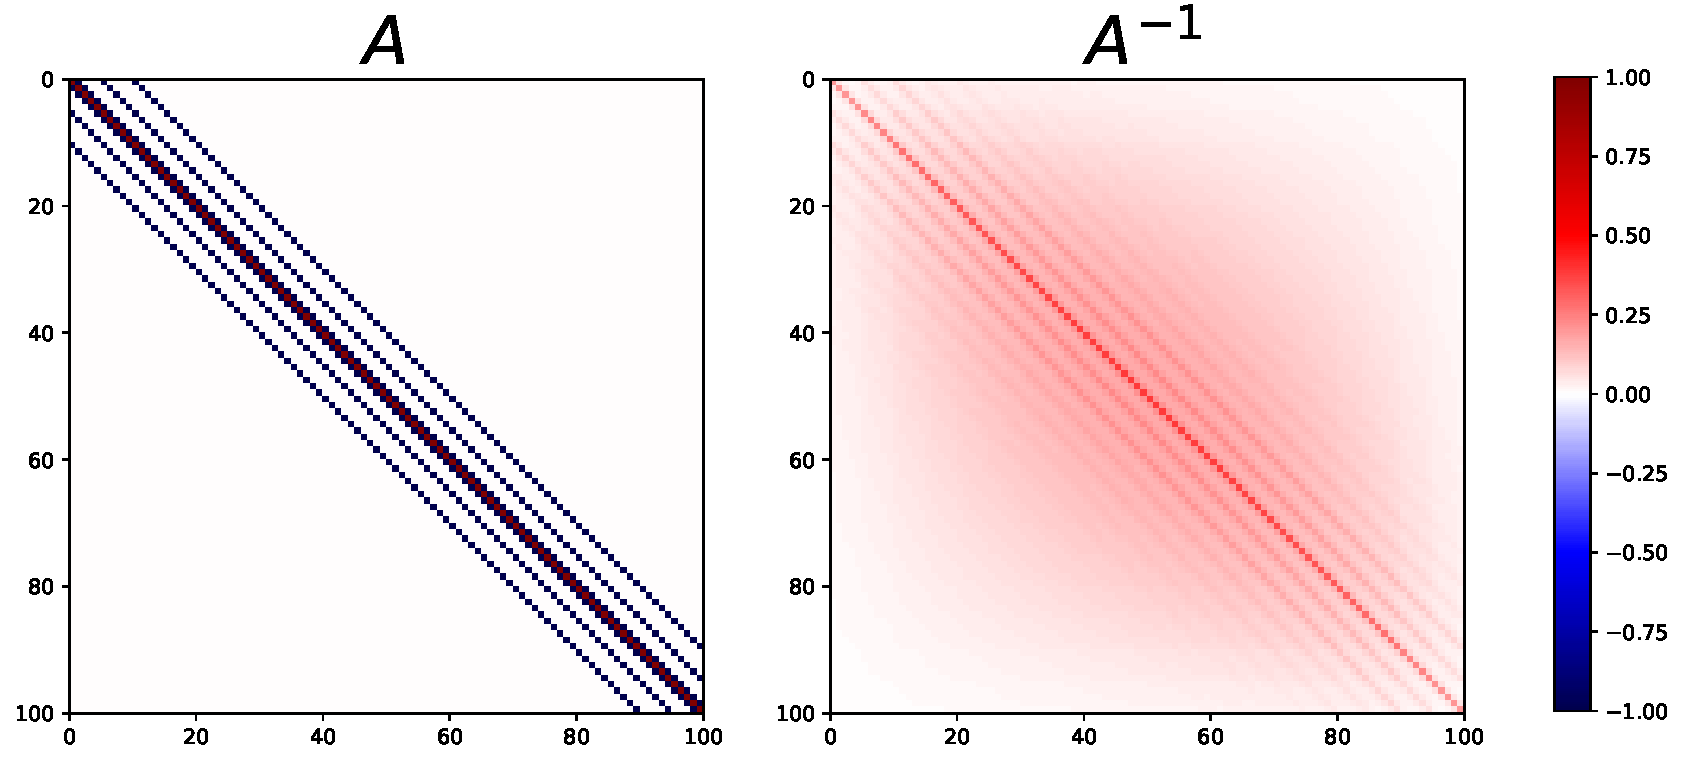
\includegraphics[width=0.8\hsize]{img/mathematical_sparsematrix.pdf}
	\caption{\(100\times 100\)の疎行列に対する逆行列のプロット。元の行列は対角成分が\(6\)、それ以外の成分が\(-1\)の行列になっている。逆行列では非ゼロ成分が全体に分布していることがわかる。ちなみにここでは逆行列がある程度綺麗な形をしているが、対角成分の値を変えると、突如奇妙な模様となる。}
	\label{fig:Math_spMat}
\end{figure}
したがって、もともとは高々700個程度の値しか保持しなくてよかったものが、逆行列ではほぼ10,000個の値を保持しなくてはならなくなってしまう。これは更に大きな疎行列では深刻な問題で、そもそも逆行列を保持するメモリの確保すら困難になる。更に、第三として逆行列自体が必要になる場合はほとんどないためである。例えば行列で表される方程式\(\boldsymbol{A}\boldsymbol{x}=\boldsymbol{b}\)の解を求める時、解は\(\boldsymbol{x}=\boldsymbol{A}^{-1}\boldsymbol{b}\)である。これを見ると逆行列\(\boldsymbol{A}^{-1}\)を求めなくてはならないようにも思えるが、実際に必要なのは\(\boldsymbol{A}^{-1}\boldsymbol{x}\)なのであって、\(\boldsymbol{A}^{-1}\)そのものではない。このようなことから、疎行列の解法では逆行列を求めずに解を求める手法が開発されている。したがって、大規模疎行列では逆行列を直接計算することは原則として行わない。

\section{一般の行列}
